\documentclass[tikz,border=10pt]{standalone}

\begin{document}

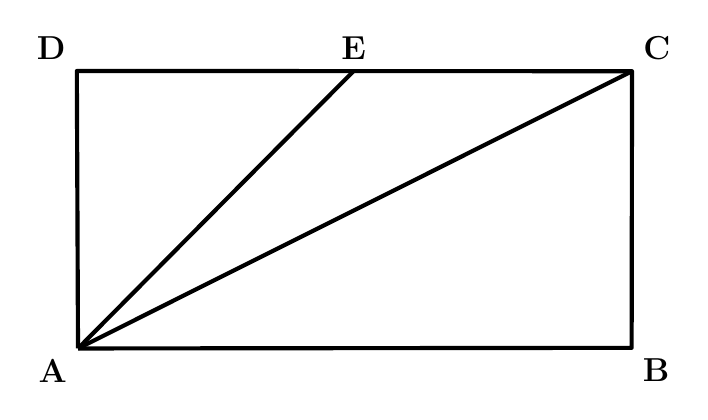
\begin{tikzpicture}[line join=round, line width=1.5pt, every node/.style={font=\fontsize{13}{15.6}\selectfont}]
\coordinate (A) at (-3.508,-1.751);
\coordinate (B) at (3.523,-1.743);
\coordinate (C) at (3.528,1.770);
\coordinate (D) at (-3.523,1.773);


  
  \coordinate (E) at (-0.008,1.772);

  
  \draw (A) -- (B) -- (C) -- (D) -- (A);

  
  \draw (A) -- (E);
  \draw (A) -- (C);

  
  \node[below left]  at (A) {$\mathbf{A}$};
  \node[below right] at (B) {$\mathbf{B}$};
  \node[above right] at (C) {$\mathbf{C}$};
  \node[above left]  at (D) {$\mathbf{D}$};
  \node[above]       at (E) {$\mathbf{E}$};
\end{tikzpicture}
\end{document}